
\documentclass[../D+Manual.tex]{subfiles}
\begin{document}

\chapter{Reciprocal Grids and the Hybrid Method} \label{chp:reciprocalGrids}
\begin{quote}
	Love is a reciprocal torture. \\
	\hspace*{\fill} \textit{Marcel Proust}
\end{quote}

\section{Background}

D+ attains its speed by first calculating the scattering amplitudes at the relevant 3D reciprocal $\vec{q}$-space of repeating subunit objects, saving them in memory, and then summing up the contribution from their multiple copies (provided by their symmetries). Using saved repeated subunit objects in memory saves the need to calculate the contribution to the scattering amplitude from each of the repeating subunits, replacing many of the calculations with lookups at the precalculated reciprocal grid (\textit{i.e.} lookup table) of the repeating subunit plus interpolation for $\vec{q}$-values between the precalculated points. As with all lookup tables, the density has to be high enough to sample all the variations and features of the scattering amplitudes. 

\begin{figure}[h!] %[12]{r}{0pt}
%	\vspace{-30pt}
\centering
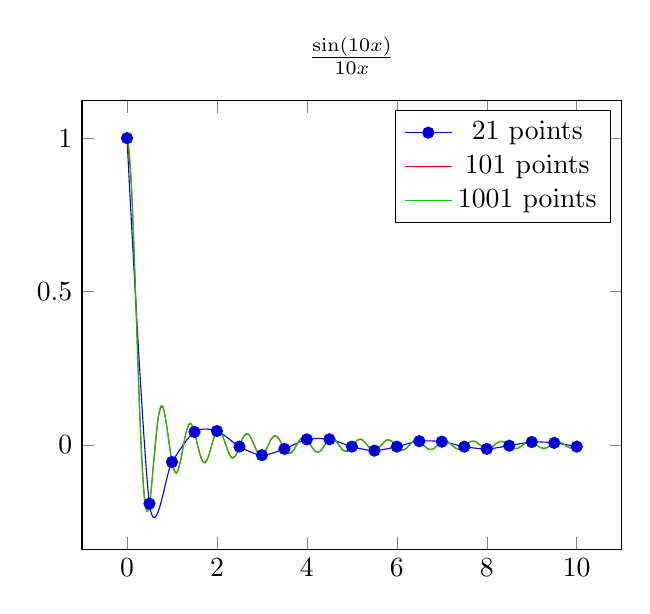
\begin{tikzpicture}
	\begin{axis} 
	[domain=0.001:10, legend, title = $\frac{\sin(10x)}{10x}$]
	%[width=190pt,axis x line=middle, axis y line=center, tick align=outside]
		%\addplot+[mark=none,smooth] (\x,{sin(\x r)});
		\addplot+[smooth, samples=21] (\x,{sin(10*\x r) / (10*\x)});
		\addplot+[mark=none,smooth, samples=101] (\x,{sin(10*\x r) / (10*\x)});
		\addplot+[mark=none,smooth,black!20!green!100, samples=1001] (\x,{sin(10*\x r) / (10*\x)});
		\legend{21 points, 101 points, 1001 points};
	\end{axis}
\end{tikzpicture}
	\caption{Plots of an oscillatory function at different sampling rates. }
	\label{fig:SamplingRate}
\end{figure}

If the largest distance within the object is $L$, the scattering amplitude will oscillate approximately like  $\sin\left(q\cdot \frac{L}{2} \right)$. The density of the points in the reciprocal-space lookup table (or grid) must be greater than two points per oscillation.
This is known as the \href{https://en.wikipedia.org/wiki/Nyquist\%E2\%80\%93Shannon_sampling_theorem} {Nyquist–Shannon sampling rate}. Hence, the grid density should be at least
	$\left(\Delta q\right)^3 \approx  \left(\nicefrac{2\pi}{L}\right)^3$ and the 3D reciprocal-space grid-size should be at least $G\approx \left(q_{\text{max}}\cdot \frac{L}{2\pi}\right)^3$, where $q_{\text{max}}$ is the maximum $q$-range.
	
Alongside the installation of D+, there is a small application dubbed \texttt{Suggest Parameters} that can be opened from the main window under the \texttt{Settings} menu. 
This application can be used to give an estimate of the necessary grid size based on the $x$, $y$, $z$, and $q_{max}$ parameters. 

As an example, consider the plots in Figure \ref*{fig:SamplingRate}.
The \textcolor{blue}{blue}, \textcolor{red}{red} and \textcolor{black!20!green!100}{green} curves all calculated $\frac{\sin\left(10x\right)}{10x}$.
The difference is only in how many points were sampled.
In the case of the blue curve, there is an under-sampling that results in inaccurate values in the regions requiring interpolation (between the blue dots).
In order to accurately represent the sinc function, the sampling density (or in our phrasing, grid density) must be increased.
The flip side is that there is little accuracy gained by increasing the sampling to 1001 points instead of 101.
Whereas the negligibly increased accuracy itself does not hurt, it costs both computation time and memory.

The Fourier space (scattering amplitude) of large repetitive objects becomes increasingly oscillatory with the size/repetitions.
Therefore, creating a reciprocal grid (from here on, RG) of the large object would require a very dense grid.
This makes na\"{\i}vely using an RG for large objects dangerous as the interpolated values will have little to do with the underlying function, just like the \textcolor{blue}{blue} curve in Figure \ref*{fig:SamplingRate}.

If the large/long object is represented by a single PDB file or a single geometric model, there is (currently) little to do.
If, however, the object is constructed of smaller repeating units, which \textit{can} be represented by an RG, there is a solution.

\subsection{Hybrid Calculations} \label{sec:hybrid}

For the Hybrid method to work, the structure must be described in a hierarchical manner.
For example, consider a series of blue spheres lined up in a linear fashion, as shown in Figure \ref*{fig:RGvsHbyrid}.
There are 12 uniform spheres of the same radius spaced $2r=\unit[2]{nm}$ apart.
%This can be shown 
Using an RG with a linear density of $\unit[0.1875]{nm^{-1}}$ (81 points between $\unit[-7.5]{nm^{-1}}$ and $\unit[7.5]{nm^{-1}}$) the scattering of single sphere can be calculated accurately.
If, however, the same RG is used to compute the scattering of all 12 spheres, then the Nyquist criteria is not met.
The resulting undersampling causes little oscillations in the generated signal with a period of the RG density, as seen in the blue curve in Figure \ref*{fig:RGvsHbyrid}.

\newsavebox{\setoftwelvespheres}
\sbox{\setoftwelvespheres}{%
    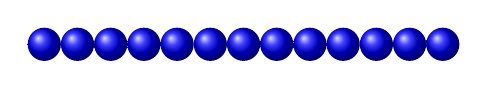
\begin{tikzpicture}%
        \foreach \z in {0,12,...,144}%
            \shade[ball color=blue] (\z pt,0) circle (6pt);%
%            \shade[ball color=blue] (0,\z pt) circle (3pt);%
    \end{tikzpicture}%
    }

\begin{figure} [h!] %[13]{r}{0pt}
	\centering
\begin{tabular}{@{}c@{}}
%\vspace{-50pt}
\hspace{20pt}
    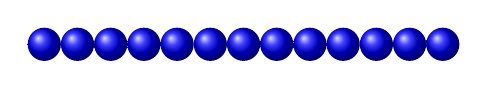
\begin{tikzpicture}%
        \foreach \z in {0,12,...,144}%
            \shade[ball color=blue] (\z pt,0) circle (6pt);%
%            \shade[ball color=blue] (0,\z pt) circle (3pt);%
    \end{tikzpicture}%
\\
%\end{figure}
%% This figure breaks the ability to compile this document separately due to the
%% lack of additional search directories in the current pgfplots (1.12). It should
%% be fixed in 1.13 as per http://tex.stackexchange.com/questions/35863/pgfplots-from-file-search-path-looking-for-graphicspath-equivalent#comment619868_35873
%\begin{figure}{r}{0pt}
	\begin{tikzpicture} %\makeatletter\let\input@path\Ginput@path\makeatother %This doesn't seem to work. Shouldn't be needed in pgfplots 1.13 when it comes out.
		\begin{axis} 
		[
		ymode=log,
		max space between ticks=20,
		yticklabels={,,},
		title={12 Spheres Spaced Evenly},
		ylabel={Intensity $\left[a.u.\right]$},
		xlabel={q $\left[nm^{-1}\right]$},	
		legend entries={With RG,Hybrid},
		]
			\addplot+[smooth,mark=none] table {HybridDemo-WithGrid.fout};
			\addplot+[smooth,mark=none] table {HybridDemo-Hybrid.fout};
		\end{axis}
	\end{tikzpicture}\\
    \end{tabular}
    \caption{Comparing the RG with the Hybrid method for the case of 12 spheres that are evenly spaced along a line.}
    \label{fig:RGvsHbyrid}
\end{figure}

There are three ways to deal with this.
The simplest and \textit{wrong} way would be to increase the RG density.
The minimal density needed is $G\approx \left(q_{\text{max}}\cdot \frac{L}{2\pi}\right)^3$ where $L$ is the largest distance within the modeled structure.
For a single sphere, $L$ is $2r$, whereas for the ensemble of twelve spheres  $L$ is $24r$.
The calculation time and memory requirements scale like $L^3$ and therefore this method is not recommended for twelve spheres.

The second way is to use the Direct method. In the Direct method, each type of geometry or PDB object is identified, and all its copies in the structure as well as their orientations and locations are collected. The intensity is then directly computed by modifying  Equation \ref{eqn:assemblyScatteringAmplitude}
so that each node in the tree structure is grouped by its orientation. If the same orientation $(j,m)$ is observed in repeating subunits in the structure, the contribution of that subunit to the total scattering amplitude is reused, with the relevant phase contribution associated with its real-space locations, given by the vectors $\vec{R}_{j,m,k}$:
	
	\begin{equation}
	\label{eqn:assemblyScatteringAmplitudeMainText}
	F\left(\vec{q}\right)=
	\sum_{j=1}^{J}
	\sum_{m=1}^{M^u_j}
	\left[F_{j}\left(\mathbf{A}_{j,m}^{-1}\vec{q}\right)\cdot
	\sum_{k=1}^{K_{j,m}}\exp\left(i\vec{q}\cdot\vec{R}_{j,m,k}\right)\right]
	\end{equation}
	
	\noindent $J$ is the number of different types of objects (leaves in the hierarchical tree, see Figure \ref{fig:hierarchical}), $M^u_j$ is the number of unique orientations of object type $j$, determined by the rotation matrices  $\mathbf{A}_{j,m}$. $K_{j,m}$ is the number of  real-space translations of object $j$ in orientation $\mathbf{A}_{j,m}$. Orientation averaging is then computed by Equation \ref{equ:OrientAvr}. In D+, the Direct method was combined with  the RG method. This combination is called the Hybrid method and it is the best solution for the case of large structures. Currently, the Direct method is implemented only for the CPU. 
	
	In the Hybrid method, RGs are computed from the leaves up to predetermined nodes in the assembly hierarchical data tree structure (Figure \ref{fig:hierarchical}), and from these nodes upward computed as subunits in the Direct method. 
	
	Differently oriented
	subunits are directly computed as in the Direct method. The highest
	calculated RGs, however, are accessed as $F\left(\mathbf{A}^{-1}\vec{q}\right)$, as in the RG method. In the Hybrid method, at least one of the leaves
	in the hierarchical data tree structure (a geometric or a PDB model) is calculated
	to an RG. RGs may be computed for internal nodes and if they are then their
	leaves are discarded and the internal nodes are treated as leaves.
	
	
	The Hybrid method averts the use of RGs that represent long structures, thus providing a solution with arbitrary accuracy in the face of the RG memory/accuracy trade-off.
	This approach is effectively a coarse-grained method with near-atomic resolution accuracy, where the subunit count ($n$) can be much smaller than the number of atoms. A rigorous analysis of the method is published in \cite{RGs2016}. The advantage of the Hybrid method is that the grid size depends on the length of the largest subunit, for which grids are calculated, rather than the length of the entire structure. Going back to our example, the preferred method is the Hybrid method in which we compute an RG for a single subunit (sphere) and use it for computing the scattering of the ensemble without an intermediate RG. More details about the algorithm can be found in \cite{RGs2016, Dplus2017}. 
\section{Using the Hybrid Method in D+}
\label{sec:UsingHybridMethod}
In practice, you can tell D+ to use the Hybrid method from a given point in a hierarchy by deselecting the \texttt{Use Grid From Here} checkbox in the \hyperref[sec:symmetryEditor]{\texttt{Symmetry Editor}} pane from the node that you do not want to use an RG.
For example, assume you wanted to model the 12 aforementioned spheres using an RG for the sphere and not for the linear spacing.
You would click on the \texttt{Sphere} in the \hyperref[sec:domainView]{\texttt{Domain View}} pane, ensuring that the \texttt{Use Grid From Here} checkbox in the \hyperref[sec:symmetryEditor]{\texttt{Symmetry Editor}} pane was checked.
You would then click on the symmetry you used to create the linear spacing in the \hyperref[sec:domainView]{\texttt{Domain View}} and uncheck the \texttt{Use Grid From Here} checkbox in the \hyperref[sec:symmetryEditor]{\texttt{Symmetry Editor}} pane.
After pressing generate a signal similar to the red curve in Figure \ref*{fig:RGvsHbyrid} will be computed.

\end{document}